\documentclass{vldb}
\usepackage{graphicx}
\usepackage{balance}  % for  \balance command ON LAST PAGE  (only there!)
\usepackage{graphicx}

\usepackage{amsmath}
\usepackage{algorithm}
\usepackage[noend]{algpseudocode}

\usepackage{caption}
\usepackage{subcaption}

\usepackage{amssymb}
\usepackage[T1]{fontenc}
\usepackage{bbm}
\usepackage{hyperref}
\usepackage[utf8]{inputenc}
\usepackage{lipsum}
\usepackage{graphicx}
\usepackage[caption=false]{subfig}
\usepackage{csvsimple}
%\usepackage{array}
\usepackage{float}
\usepackage{amsmath}
\usepackage{pgfplotstable}

\usepackage{algorithm}
\usepackage[noend]{algpseudocode}
\usepackage{varwidth}

\begin{document}

% ****************** TITLE ****************************************

\title{LDA Model Monitoring in Distributed Systems}


\numberofauthors{3} %  in this sample file, there are a *total*
% of EIGHT authors. SIX appear on the 'first-page' (for formatting
% reasons) and the remaining two appear in the \additionalauthors section.
%
\author{
% You can go ahead and credit any number of authors here,
% e.g. one 'row of three' or two rows (consisting of one row of three
% and a second row of one, two or three).
%
% The command \alignauthor (no curly braces needed) should
% precede each author name, affiliation/snail-mail address and
% e-mail address. Additionally, tag each line of
% affiliation/address with \affaddr, and tag the
% e-mail address with \email.
%
% 1st. author
\alignauthor
Ran Bernstein\\
       \affaddr{Technion -- Israel Institute of Technology}\\
       \affaddr{Haifa 32000 Israel}\\
       \email{bernstein.ran@Gmail.com}
% 2nd. author
\alignauthor
 Daniel Keren\\
       \affaddr{University of Haifa}\\
       \affaddr{Haifa 31905 Israel}\\
       \email{dkeren@cs.haifa.ac.il}
% 3rd. author
\alignauthor
Margarita Osadchy\\
       \affaddr{University of Haifa}\\
       \affaddr{Haifa 31905 Israel}\\
       \email{rita@cs.haifa.ac.il }
\and  % use '\and' if you need 'another row' of author names
% 4th. author
\alignauthor Assaf Schuster\\
       \affaddr{Technion -- Israel Institute of Technology}\\
       \affaddr{Haifa 32000 Israel}\\
       \email{assaf@cs.technion.ac.il}
}

\date{30 March 2016}

\maketitle

\begin{abstract}
Real systems for mining dynamic data streams should be able to detect changes that affect the accuracy of their model. A distributed setting is one of the main challenges in this kind of change detection. In a distributed setting, model training requires centralizing the data from all nodes (hereafter, synchronization), which is very costly in terms of communication. In order to minimize the communication, a monitoring algorithm should be executed locally at each node,
while preserving the validity of the global model (the model that will be computed if a synchronization will occur). For minimizing this communication, we propose the first communication-efficient algorithm for monitoring a classification model over distributed, dynamic data streams. The classification algorithm that we chose to monitor is Linear Discriminant Analysis (LDA), which is a popular method used for classification and dimensionality reduction in many fields. This choice was made due to the strong theoretical guarantee of correctness that we prove on the monitoring algorithm of this kind of model.
In addition to its theoretical guarantee, it is shown empirically that our algorithm reduce communication volume by up to two orders of magnitude (compared to synchronization in every round) on three real data sets from different worlds of content. Moreover, our approach monitors the classification model itself as opposed to its misclassifications, which makes it possible to detect the change before the misclassification occurs.
\end{abstract}

\section{Introduction}
\label{intro}
In this work, we address the problem of mining data streams when the data is
{\em distributed} over a large number of nodes with the same data generation process at every node. However, the streaming data is not stationary; notably, it can change over time. Classic examples of real-life prediction problems that involve this kind of change are user preference prediction and fraud detection. In the former, the choices of the user can change over time; in the latter, the fraudulent transactions change constantly to avoid detection. In both, the change can render the prediction model invalid.
In such a setting --- where the model must be updated to stay valid and communication is costly --- the question is \textit{when} to recompute the model. The naive solution for this problem is recomputing the model periodically. The problem with this solution is that it involves needless work if the model changes infrequently, yet may introduce unacceptable errors between scheduled updates. 
In contrast to periodical computation, we focus on \textit{monitoring} the quality of a given model, and recomputing it only as needed. 
\par We focus on linear binary classifiers, using LDA \cite{fisher1936use} as the learning algorithm. This choice is due the popularity of linear classifiers in real applications and that they serve as a platform for more complex classifiers, such as ensemble model in the work of ~\cite{Deva, eSVM}, neural networks in the work of ~\cite{osadchy2015k}, and even deep architectures in the work of \cite{ROSS}. Our method is distinct from the previous work in the following two aspects:

\noindent \textbf{Model-Based Monitoring:} 
Monitoring the model and not the misclassifications has an important benefit: the need for synchronization can be detected before the misclassifications occurs. In contrast to most previous work on monitoring a classifier (that utilizes misclassification rates to draw conclusions about the change in the distribution ~\cite{baena2006early,gama2004learning,Nishida2007}), we propose to monitor the change in the {\em model} itself.

\noindent \textbf{Distributed Setting:} Monitoring a classifier has been actively studied in centralized settings. In contrast to these studies, our is one of the very few works that monitor in a distributed setting. In such setting, data is distributed over a large number of nodes and the model is learned globally after synchronization. While the few existing methods for classifier monitoring in distributed settings rely on heuristics (~\citealt{AngGZPH13}), our approach is the only one that provides a provable guarantees of correctness.

\section{Related Work}
Monitoring dynamic data streams is a broad topic that has been addressed in different research communities. Within this field, we focus on detecting a change in the data stream that renders the prediction model invalid. 
In distributed settings, this problem is even harder and referred to as {\em distributed monitoring}, and it is concerned with designing local tests for monitoring a function that is defined globally over all the nodes in the system.
Our approach to this problem is to define a constraint over the local data (at each node) that guarantees the validity of the global model. If local data (in one or more nodes) does not meet the local condition, it leads to synchronization. The synchronization process has large communication costs, and the goal of the distributed monitoring methods is thus to minimize the number of synchronizations. Most of the work on distributed monitoring has been concerned with simple functions of the data, such as linear functions in the work of ~\cite{keralapura2006communication} and ~\cite{kashyap2008efficient} or monotonic functions in the work of \cite{michel2005klee}.
For non-linear functions, examples include work on monitoring the value
of a single-variable polynomial as in the work of ~\cite{shah2008handling},
and eigenvalue perturbation as in the work of ~\cite{huang2007communication}.
While the previous work handled specific families of functions, we chose to use \textit{geometric} approach for monitoring \textit{arbitrary} functions over distributed streams, as was proposed, later extended and generalized in \cite{sharfman2007geometric, keren2014geometric, keren2012shape}. A recently introduced work by ~\cite{gabel2015monitoring} on monitoring Least Square Regression (LSR) using geometric monitoring is the closest to ours, but our problem is more complex: unlike the global scatter matrix (required by LSR) the global covariance matrix (required in LDA) is not the mean of the local covariance matrices which makes the monitoring problem more much harder.

\section{Problem Definition}
We first describe the Linear Discriminant Analysis (LDA) algorithm and then define the monitoring problem. 

\subsection{Linear Discriminant Analysis}%\\ \par
LDA seeks a linear combination of features that characterize or separate two or more classes of samples.
The resulting combination may be used as a linear classifier, or for dimensionality reduction before later classification.

In LDA the problem is approached by assuming that the conditional probability
density functions $Pr(\vec x|y=p)$ and $Pr(\vec x|y=q)$ are both normally distributed with
mean and covariance parameters $(p, B_p)$ and
$(q, B_q)$, for two target classes P and Q respectively.
${(x_1,y_1),\ldots,(x_n,y_n)}$ are i.i.d. samples, $x_i \in \mathbb{R}^d$
and $y_i \in \{0,1\}$.

We seek a linear transformation (model), $w \in \mathbb{R}^d $,
that maximizes the separation between the classes, where the separation is
defined to be the ratio of the variance between the classes to the variance
within the classes:
\begin{equation}
S := \frac{\sigma^2_{between}}{\sigma^2_{within}} = \frac{(w^T (p -
q))^2}{w^T(B_p+B_q)w}.
\end{equation}
Solving the maximization problem yields that the decision criterion is a threshold on the
dot product
\begin{equation*} \label{eq:decision}
w \cdot x > c
\end{equation*}
where
\begin{equation} \label{eq:w}
w \propto (B_p+B_q)^{-1}(p - q)
\end{equation}
\begin{equation} \label{eq:c}
c = \frac{1}{2}(T-{p}^T S_p^{-1} {p}+{q}^T S_q^{-1} {q}).
\end{equation}
In this work we monitor $w$, and will refer it as the classification \textit{model}.

\subsection{Monitoring Problem}
We denote $k$ as the number of nodes and $W$ as the number of samples in a node.
Our model uses discrete time (hereafter, rounds). Every node receives a new sample
in a round. We use the \textit{sliding window} model, every node keeps two sliding windows (one for each class) of length of $W/2$. As a node receives a new observation, it replaces the oldest one from its class.
$x^i_j$ and $y^i_j$ are the $j$'th sample and label in the $i$'th node
and $x_{old}^i(p)$ and $x_{old}^i(q)$ are the oldest samples from each class in
the sliding window of the $i$'th node.
As data evolves, it is possible that the previously computed model
no longer matches the current true model. Let $w_0$ be the existing model (vector of weights of a linear classifier), previously computed at some point in the past (the synchronization time), and let $w$ be the \textit{true} LDA model (the hypothetical model that synchronization would yield if it occur).
We wish to maintain an accurate estimation $w_0$ of the current global LDA model, $w$.
For the classification purpose, the most important property of a linear classifier is its direction. Therefore, we monitor the change in this direction: given a threshold $T$, our goal is to raise an alert if
\begin{equation} \label{eq:coneCritiria}
\frac{<w,w_0>}{\parallel w \parallel \parallel w_0 \parallel}  < T.
\end{equation}
i.e. if the angle between $w0$ and $w$ is above a certain threshold (inner product between unit vector is the $cosine$ of the angle between them).

%Due to the complexity of Eq. \ref{eq:coneCritiria},
%we will monitor a simpler problem whose solution also satisfies
Due to the complexity of condition \ref{eq:coneCritiria}, we will monitor a restriction of it: we replaced the cone containment condition to a  sphere containment condition, i.e., 
%Eq. \ref{eq:coneCritiria}: the maximal volume sphere of which $w_0$ is its center
%that resides completely inside the cone from Eq. ~\ref{eq:coneCritiria}.
%This sphere is defined by
\begin{equation} \label{eq:critiria}
||w-w_0||   >  R_0,
\end{equation}
where $R_0 := ||w_0|| \sqrt{1-T^2}$ is the radius of the maximal volume sphere of which $w_0$ is its center and resides inside the cone from condition \ref{eq:coneCritiria}.
%In other words, we replaced containment by distance from the boundary.
%Empirical evaluation showed that the values of
%$1-\frac{<w,w_0>}{||w||||w_0||}$ and $||w-w_0||$ are
%highly  correlated, thus in practice, Eq. \ref{eq:coneCritiria}
%can be replaced by Eq.\ref{eq:critiria}.


\section{Monitoring Distributed LDA With Convex Subsets}
Monitoring distributed LDA models is difficult because the
global model cannot be inferred from the local model at each
node. Even when all current local models $w_i$ are similar to the precomputed
local models $w_0$, the current global model $w$ may
be very different from the precomputed model $w_0$
\footnote{Note that this has the obvious benefit of preserving the privacy
of the data in each node from all the other nodes.}.
Consider the example in Figure \ref{NegativeExample} with $k = 2$ nodes
and dimension $d =2$.
The angle deviation of the global model (shown in solid lines) is large (45 degrees)
even though the local models (shown in dashed lines) are identical to what they
were at the initial point.

\begin{figure}[h]
\centering
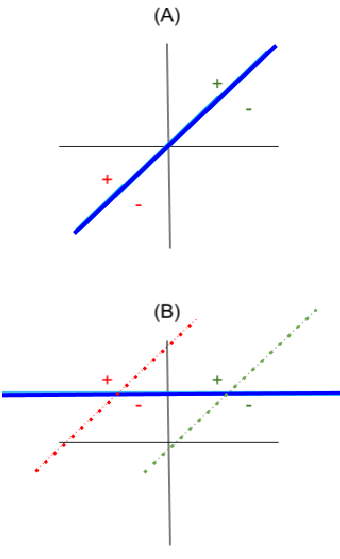
\includegraphics[width=60mm, height=9cm]{NegativeExample.png}
\caption{Example of incorrect monitoring by applying LDA locally. The
initial state of the data is presented in (A) and the state at a later point
is shown in (B). In (B) every node (green and red dashed lines) calculates the same angle
for the separator as it was in (A). But it can be
seen that the global separator's (blue solid line) angle has changed
significantly.}
\label{NegativeExample}
\end{figure}


\par To overcome this difficulty, we turn to geometric monitoring. Geometric
monitoring such as in the works of \cite{keren2014geometric, keren2012shape} is a communication
efficient approach that monitors whether a function of distributed
data streams crosses a threshold. The key idea is to
impose constraints on local data at the nodes, rather than
on the function of the global aggregate. Given a function of
the average of all local data and the threshold, we compute a
``good'' convex subsets, called \textit{safe zones}, for each
node.

\par As we show below, convexity
plays a key role in the correctness of this scheme. As long
as local data stay inside the safe zones, we guarantee that
the function of the global average does not cross a threshold (given
in terms of maximal angle or norm of distance between the classifiers).
Nodes communicate only when local data leaves the
safe zone, which we call a safe zone \textit{violation} (hereafter,
violation). Once that happens, violations can be resolved,
for example by aggregating data from all the nodes and recomputing $w_0$
and the safe zones (synchronization).
In other words, we want to impose conditions on the local
data at each node so that as long as they hold, $||w-w_0||<R_0$.

\subsection{Notation}
\noindent
$P$ and $Q$ are the classes in the binary classification problem.
 $(p,q)$ and $(p^i,q^i)$  are the global and local means of classes $P$ and $Q$.
\\$S$ and $S^i$  are the global and local normalized scatter matrices of the feature space:
\begin{equation*}
S^i := \frac{1}{n}\sum_{j=1}^{n}x^i_j(x^i_j)^T
\end{equation*}
\begin{equation*}
S := \frac{1}{nk}
\sum_{i=1}^k\sum_{j=1}^nx^i_j(x^i_j)^T=\frac{1}{k}\sum_{i=1}^kS^i.
\end{equation*}
\\Similarly, $u$ and $u^i$ are the distance between the means of the classes, i.e., $u:=p - q$ and $u^i:=p^i - q^i$.
\\ $B$ is the global covariance matrix, which is the sum of the covariance matrices of the two classes, i.e., $B:=B_p+Bq$.
It can be shown that $B=S - pp^T - qq^T$.
%\\B^i:=S^i - p^i(p^i)^T - q^i(q^i)^T$
\\Let w be our current true model. Then, following Eq.~\ref{eq:w}, we can express:
%\\$w(S,\mu_p,\mu_q) := (S - \mu_p\mu_p^T - \mu_q\mu_q^T)^{-1}(\mu_p - \mu_q)$
\begin{equation}
w:=(S - pp^T - qq^T)^{-1}(p-q)=B^{-1}u.
\end{equation}
%In the following the subscript $0$ will denote the state at the time
%of last synchronization.
Let $w_0$ be the existing model, previously computed from $(S_0, p_0, q_0)$
or from $(B_0,u_0)$ at the time of synchronization.
Then,
\begin{equation}
w_0:=(S_0 - p_0p_0^T - q_0q_0^T)^{-1}(p_0-q_0)=B_0^{-1}u_0.
\end{equation}
$\Delta_s, \delta_p$, and $\delta_q$ are the global drift vectors of $S, p$, and $q$,
i.e.,
\begin{alignat*}{1}
& \Delta_s:= S - S_0 \\
& \delta_p:= p - p_0 \\
& \delta_q := q - q_0.
\end{alignat*}
\\If $S_0^i$, $p_0^i$ and $q_0^i$ are the local normalized scatter and averages
of the samples in a node, we can define the local drifts to be:
\begin{alignat*}{1}
& \Delta_s^i:= S^i - S_0^i
\\ & \delta_p^i:= p^i - p_0^i
\\ & \delta_q^i:= q^i - q_0^i.
\end{alignat*}
\begin{remark} \label{average}
It is easy to see that every global drift vector is the average of the local drift vectors:
\begin{alignat*}{1}
& \Delta_s = \frac{1}{k} \sum \Delta_s^i, \\
& \delta_p = \frac{1}{k} \sum \delta_p^i, \\
& \delta_q = \frac{1}{k} \sum \delta_q^i.
\end{alignat*}

\end{remark}

\subsection{Convex Safe Zones}
Each node monitors its own drift vector: as long as current values
at local nodes $(S^i,p^i,q^i)$ are sufficiently similar to their values
at synchronization time $(S^i_0,p^i_0,q^i_0)$, $w_0$ is guaranteed to be close to $w$.
Formally, we define a convex set $\mathcal{C}$ such that:
\begin{equation} \label{convex}
(\Delta_s, \delta_p, \delta_q) \in \mathcal{C} \Rightarrow \parallel w-w_0
\parallel \ < R_0.
\end{equation}
\begin{lemma} \label{averages}
Let $\mathcal{C}$ be a convex set that satisfies Eq. \ref{convex}.
If $(\Delta_s^i, \delta_p^i, \delta_q^i) \in \mathcal{C}$ for all i, then
\begin{equation*}
||w-w_0|| < R_0.
\end{equation*}
\end{lemma}
\begin{proof}
We express $S, p$ and $q$ as their values at synchronization with the addition of the average of the local drift vectors:
\begin{equation}
\begin{split}
\\(S,p,q) & = \frac{1}{k} \sum_i (S^i,p^i,q^j) \\
 & = (S_0,p_0,q_0) + \frac{1}{k} \sum_i (\Delta_s^i,\delta^i_p,\delta_q^i). \\
\end{split}
\end{equation}
From $\mathcal{C}$'s convexity and using Remark \ref{average} we get:
\begin{equation}
\begin{split}
\forall i (\Delta_s^i,\delta^i_p,\delta_q^i) \in \mathcal{C} & \Rightarrow
\frac{1}{k} \sum_i (\Delta_s^i,\delta^i_p,\delta_q^i) \in \mathcal{C} \\
& \Rightarrow (\Delta_s,\delta_p,\delta_q) \in \mathcal{C}.
\end{split}
\end{equation}
Finally, from the definition of $\mathcal{C}$ we obtain:
\begin{equation}
(\Delta_s,\delta_p,\delta_q) \in \mathcal{C} \Rightarrow \parallel w-w_0
\parallel \ < R_0,
\end{equation}
\end{proof}

\subsection{Convex Bound for Local Condition}
We denote the change in the global covariance matrix
\begin{alignat*}{2}
\Delta & := && B-B_0 \\
& = && (S_0+\Delta_S - (p_0+\delta_p)(p_0+\delta_p)^T \\
& && - (q_0+\delta_q)(q_0+\delta_q)^T) \\
& && - (S_0 - p_0p_0^T - q_0q_0^T) \\
& = && - \delta_p\delta_p^T - \delta_q\delta_q^T \\
& && + \Delta_S - p_0\delta_p^T \\
& && - \delta_pp_0^T - q_0\delta_q^T - \delta_qq_0^T.
\end{alignat*}
We break $\Delta$ into its quadratic part,
\begin{equation*}
M:= - \delta_p\delta_p^T - \delta_q\delta_q^T
\end{equation*}
\begin{equation*}
M^i:= - \delta_p^i(\delta_p^i)^T - \delta_q^i(\delta_q^i)^T
\end{equation*}
and its linear part,
\begin{equation*}
L:= \Delta_S - p_0\delta_p^T - \delta_pp_0^T - q_0\delta_q^T - \delta_qq_0^T
\end{equation*}
\begin{equation*}
\\ L^i := \Delta_S^i - p_0^i(\delta_p^i)^T - \delta_p^i(p_0^i)^T -
q_0^i(\delta_q^i)^T - \delta_q^i(q_0^i)^T,
\end{equation*}
and hence
\begin{equation*}
\Delta= L+ M, 
\end{equation*}
\begin{equation*}
\Delta^i:= L^i+ M^i.
\end{equation*}
We denote the change of the distance between the means as
\begin{equation*}
\delta:= u-u_0 = \delta_p - \delta_q, 
\end{equation*}
\begin{equation*}
\delta^i:=\delta_p^i - \delta_q^i.
\end{equation*}
Now we can state a convex bound for our problem:
\begin{lemma} \label{convexBound}
Let $\mathcal{G}$ be the set of triplets $(\Delta_s^i, \delta_p^i, \delta_q^i)$
 that satisfies the bound:
 \begin{equation} \label{eq:convexBound}
||B_0^{-1}\delta^i|| + (||w_0||+R_0)(\Big \| B_0^{-1}L^i \Big \| + \Big \| B_0^{-1}M^i \Big \| ) \leq  R_0
\end{equation}
where $\Big \| A \Big \|$ is the operator norm of the matrix $A$, and $||v||$ is the euclidean norm of the vector $v$.
\\If $\Big \| B_0^{-1}\Delta^i \Big \| < 1$, then $\mathcal{G}\subseteq \mathcal{C}$ and $\mathcal{G}$ is convex.
\end{lemma}
The proof of Lemma \ref{convexBound} and the definition for operator norm are given in Appendix A.

\section{Method}
In the following, we present two frameworks for LDA model monitoring that use
the bound in Eq. \ref{eq:convexBound}. 
In both frameworks, 
we define a \textit{coordinator}, whose role is to monitor the violation alerts from the nodes and aggregate the data from all the nodes when it happens. The coordinator recomputes the model after data aggregation and sends the new covariance matrix and the norm of the new model to the nodes (in privacy preserving mode, the coordinator is a trusted party).
In both frameworks every node runs the same
update algorithm as detailed in Alg. \ref{NodeUpdate}.
The frameworks differ in their synchronization policy. 
The first, Distributed LDA Monitoring (DLDA), will synchronize in a round
in which at least one node has reported a violation as detailed in Alg.~\ref{DLDA}).
The second, Probabilistic Distributed LDA Monitoring (PDLDA), will synchronize in a round in which the number of nodes with a violation is above a certain
threshold.
The derivation of this threshold is presented Section \ref{sec:PDLDA}.


\begin{algorithm}
\caption{Node Update: $i$ is the index of the node, $(x,y)$ is a new sample.}
\label{NodeUpdate}
\begin{algorithmic}[1]
\Procedure{Update}{}
\If {$y$ is class P}
\State $p^i = p^i + x - x_{old}^i(p)$
\State $S^i = S^i +xx^T - x_{old}^i(p)*(x_{old}^i(p))^T$
\Else
\State $q^i = q^i + x -x_{old}^i(q)$
\State $S^i = S^i +xx^T - x_{old}^i(q)*(x_{old}^i(q))^T$
\EndIf
\State $(\Delta_s^i,\delta^i_p,\delta_q^i) = (S^i-S^i_0,p^i-p^i_0,q^i-q^i_0)$
%\If{The bound in \ref{eq:convexBound} is not satisfied}

\If { \begin{varwidth}[t]{\linewidth}
$||B_0^{-1}\delta^i||+ (||w_0||+R_0)(||B_0^{-1}L^i||+||B_0^{-1}M^i||) $ \par
\hskip\algorithmicindent $>R_0$}
\end{varwidth}
\State Report violation to coordinator
\State Receive new global $B_0^{-1}$, $||w_0||$
\State $(S_0^i,p_0^i,q_0^i) = (S^i,p^i,q^i)$
\EndIf

\EndProcedure
\end{algorithmic}
\end{algorithm}

\begin{algorithm}
\caption{Coordinator synchronization algorithm.}\label{DLDA}
\begin{algorithmic}[1]
\Procedure{Sync}{}
\If {One of the nodes has reported for violation}
\State Receive from every node $i$ the triplet $(S^i,p^i,q^i)$
\State Compute updated $||w_0||$ and $B_0^{-1}$ and distribute.
\EndIf
\EndProcedure
\end{algorithmic}
\end{algorithm}

\subsection{Probabilistic Distributed LDA Monitoring}\label{sec:PDLDA}

DLDA triggers synchronization when a single node reports a violation.
Our empirical evaluation with a large number of nodes showed that such a strict
policy causes synchronization when the global model is still valid. The likely
reason for this phenomenon is that the theoretical bound is not tight enough.
To resolve this problem, we suggest relaxing the synchronization policy of
the system and synchronizing when a certain portion of nodes report a violation.
Next, we derive a threshold on the number of nodes with violations; this threshold indicates that the euclidean distance between the true global model to the one that was computed in the last synchronization (hereafter, model drift) is greater than the permitted level.
To compensate for relaxing the threshold on the number of violated nodes
(from 1), we lower it on the model change: $\|w-w_0\| \geq R_0$
to $u<R_0$.

Let $U\in\{0,1\}$ be an indicator variable, such that $U=1$,
when $\|w-w_0\| \geq u$ and $U=0$ otherwise (now, $U=1$ indicates the concept drift).
Let $v_i \in \{0,1\}$ be an indicator for a violation in the
$i$'th node. We define the probability for local violation in a node given $U=0$ as:
\begin{alignat*}{1}
%& P_{TP} := P(v_i=1 | U=1) \\
& P_{FP} := P(v_i=1 | U=0).
\end{alignat*}
Let $V$ be the random variable denoting the number of violations
\begin{equation*}
V := \sum_{i=1}^k v_i.
\end{equation*}

We denote the minimal number of violations that cause a synchronization
as a \textit{violation threshold} $t$, and it is quantified by
$t:=k*P_{FP}+z$ for some integer $z$.
We would like to find $z$ for deriving a condition that, for a given $0 < \epsilon < 0.5$,
guarantees that
$P(V>t|U=0) < \epsilon$.
\\From the Chernoff bound it follows that
\begin{alignat*}{1}
& P(V>t | U=0) \\
& = P(V>k*P_{FP}+z | U=0) \\
& \leq \exp(-\frac{z^2}{2kP_{FP}(1-P_{FP})}) \\
& \leq \epsilon.
\end{alignat*}
For $z^*:=\sqrt{2kP_{FP}(P_{FP}-1)\log(\epsilon)}$ the condition is satisfied.
Consequently, for $t^*:=k*P_{FP}+z^*$,  $P(V > t^*|U=0) < \epsilon$.
We found a threshold $t^*$ on the number of nodes with violations, such that if $V > t^*$,  then
$\|w-w_0\| \geq u$ with high probability, and thus synchronization is required.

\section{Evaluation}
\begin{figure*}[ht]
	\centering
	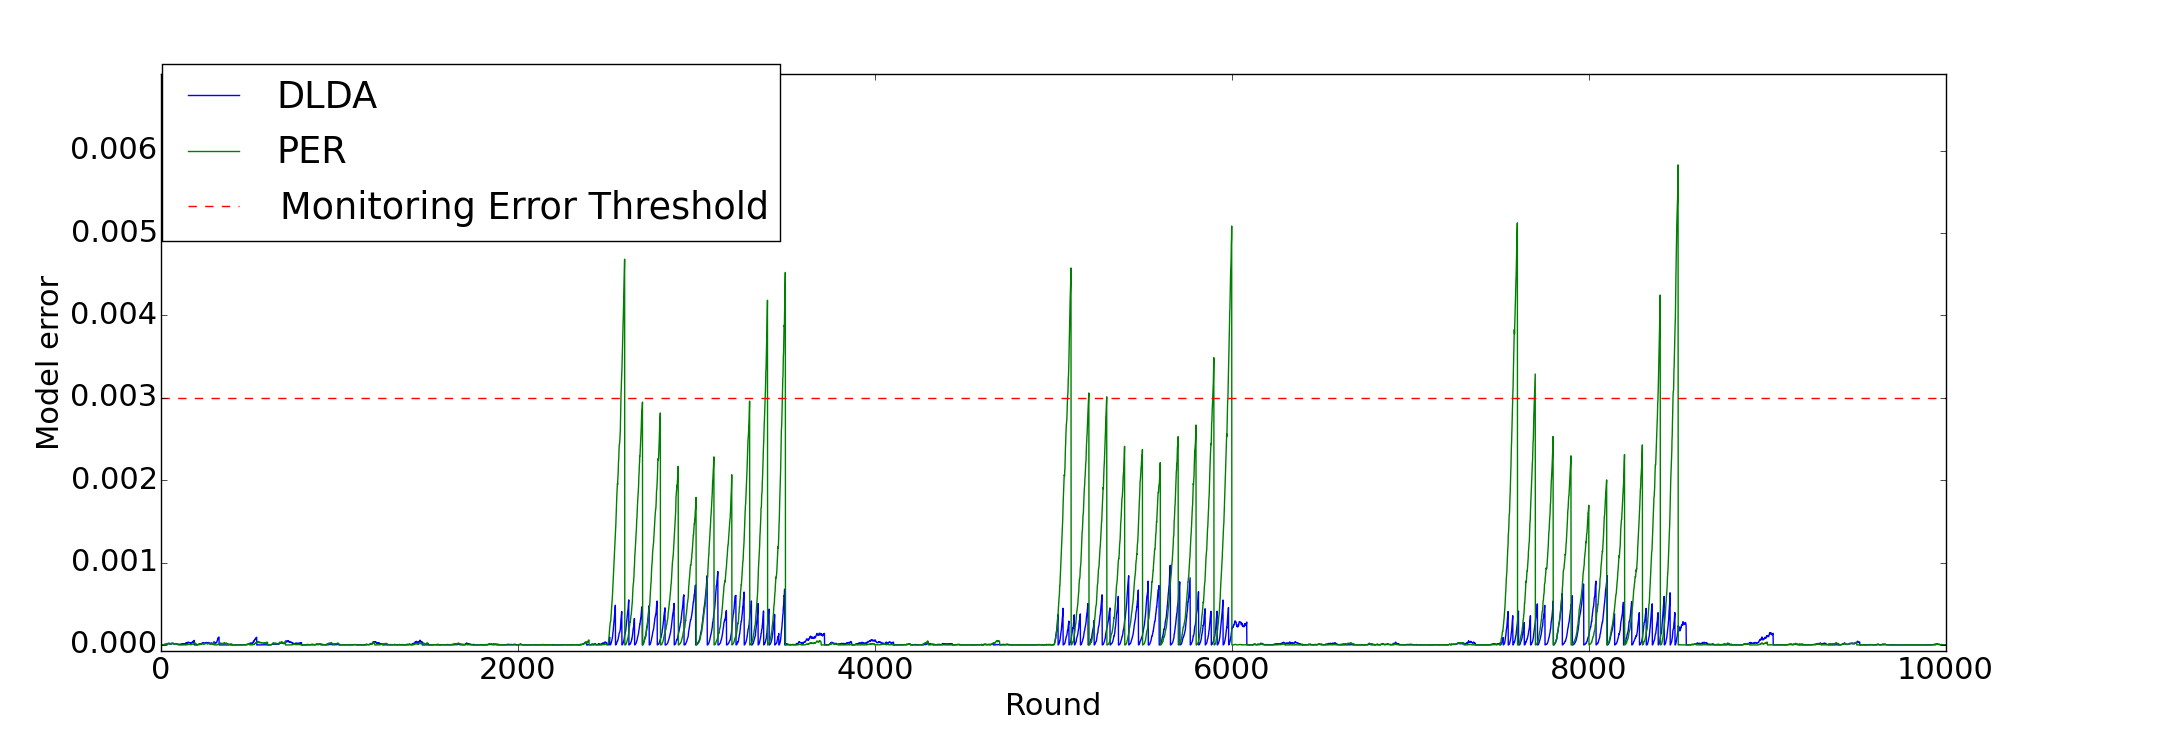
\includegraphics[width=\textwidth, height=5cm]{PER/PERvsDLDAoverTime.png}
	\caption{ DLDA (blue) model error (1 - $\frac{<w_0,w>}{||w||||w_0||}$) compared to PER(100) model error (green),
	for k = 10 simulated nodes with d = 2 dimensions, threshold T = 0.997 and
	window size L=1000. Both algorithms reduce communication to 1\%, but DLDA
	only synchronizes when $w$ changes. PER(100) synchronizes every 100 rounds,
	but is unable to maintain model error below the threshold (dashed horizontal line).}
	\label{PERvsDLDAoverTime}
\end{figure*}

We evaluated the performance of the proposed monitoring algorithms,
DLDA and PDLDA, on synthetic and real
data. For each dataset we simulated a distributed data stream by partitioning the data between the nodes and streaming it one sample in a round. 

\subsection{Synthetic Data Experiments}
We use synthetic data, in which all model assumptions hold, to
exemplify the communication efficiency of our method (Section \ref{sec:com_eff}) and its ability to detect a concept drift before the misclassifications (Section \ref{sec:earlydetection}). We then (Section \ref{sec:paramanal}) analyze the communication efficiency of our method as a function of algorithm parameters.

\subsubsection{Communication Efficiency}\label{sec:com_eff}
We compare DLDA to the T-periodic algorithm, denoted
PER(P), which is a simple sampling algorithm that sends updates
every P rounds.
Our main performance metric is communication, measured
in \textit{normalized messages} (the average number of messages sent per
round by each node). PER can achieve arbitrarily low communication at the cost of larger model drift. Periodic synchronization can miss the point of change in the data; hence it cannot guarantee to maintain the model drift under a fixed threshold, in contrast to DLDA.  DLDA has additional intrinsic advantages over PER: 1) DLDA can be instantly calibrated to fit a given drift threshold, while for PER the interval between synchronizations can only be determined empirically, which is slower. 2) Contrary to PER, DLDA does not require an adaptation period when the rate of the concept drift changes. 3) For a sudden concept drift, DLDA adapts immediately --- the algorithm's \textit{latency} is 0 --- while for PER the latency might be up to the period length.
%1) For a given allowed error rate, DLDA can be immediately calibrated not to exceed it while for PER the right period has to be found empirically.
%2) If the rate that the date evolves changes, PER won't adapt its period size,
%while DLDA adapts immediately.
	
Figure \ref{PERvsDLDAoverTime} shows the behavior of the DLDA monitoring
algorithm over a synthetic dataset with 3 concept drifts.
DLDA achieves communication of 0.01 messages per node per round, and
the model error $(1 - \frac{<w_0,w>}{||w||||w_0||})$ and thus the model drift  is always below the given threshold.
Conversely, the equivalent PER(100) algorithm doesn't maintain the
model error below the threshold (red dashed line).
Figure \ref{PERvsDLDAoverTime} shows that the periodic algorithm does not always  synchronize when the model drift exceeds a given threshold. Moreover, it  triggers redundant synchronizations when there is no concept drift.

\subsubsection{Early Drift Detection}\label{sec:earlydetection}
\begin{figure*}[ht]
	\centering
	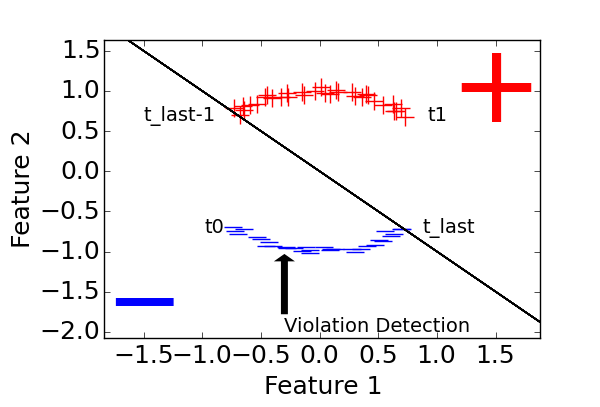
\includegraphics[width=120mm, height=5cm]{EarlyDetection.png}
	\caption{A toy example for early concept drift detection. The positive class samples are shown as pluses and the negative class samples are shown as minuses. The changes in both classes follow a 2D arc in opposite directions. $t_0, t_1$ are the first samples from the two classes; $t_{last-1}, t_{last}$ are the last (chronologically) samples from the two classes. The first violation is reported at the sample with an arrow on it, which happens prior to the first misclassification (in the  last sample $t_{last}$) that ended the experiment.}
	\label{EarlyDetection}
\end{figure*}
Consider a toy example (see Figure \ref{EarlyDetection}), in which 2D data arrives from two classes (the positive class samples are shown as pluses and the negative class samples are shown as minuses), each one following a 2D arc in the opposite direction. The class is switched at each round. Both classes exhibit a concept drift towards the separation boundary, which eventually crosses it, causing a misclassification (at time $t_{last}$). We apply the DLDA method to detect the concept drift, and it detects it prior to the time (with some margin) when the missclassification occurs (see the point of the first violation alert in Figure \ref{EarlyDetection}). This example demonstrates an important advantage of our method over misclassifications-based concept drift detection methods, which detect concept drift only after the model becomes inaccurate or invalid.

\subsubsection{Parameter Analysis}\label{sec:paramanal}
Next, we analyze the parameters of the DLDA algorithm.

\noindent\textbf{Model Drift Threshold:} Model Drift Threshold is given by the user. Above it the model drift is too big. It can be quantified in two ways: as the maximal angle between $w$ and $w_0$, or as the euclidean distance between them. 
Figure \ref{PERvsDLDAoverError} shows the communication requirements of the DLDA algorithm as a function of the model drift threshold, and the minimal communication required to match DLDA using PER.	
It can been seen that for both fixed and dynamic data, DLDA outperforms PER for
any given model drift threshold.
 \begin{figure*}[ht]
	\centering
	\includegraphicswidth=120mm, height=5cm]{PER/onlyDrift.png}
	\caption{Communication as the function of model drift for DLDA and PER. The
	periodic algorithm is tuned to achieve the same max model drift as DLDA
	for each model drift threshold.}
	\label{PERvsDLDAoverError}
	\end{figure*}

	
\noindent\textbf{Node Scalability:}
Node Scalability is how DLDA performs with different number of nodes.
Figure \ref{Nodes} shows the communication volume as a function of the number of nodes $k$.
We observe that communication increases slowly, reaching 0.25\% on the fixed
data and 0.6\% on the dynamic data distributed across 25 nodes.

\begin{figure}[!htb]
\centering
\minipage{0.4\textwidth}
    \centering
  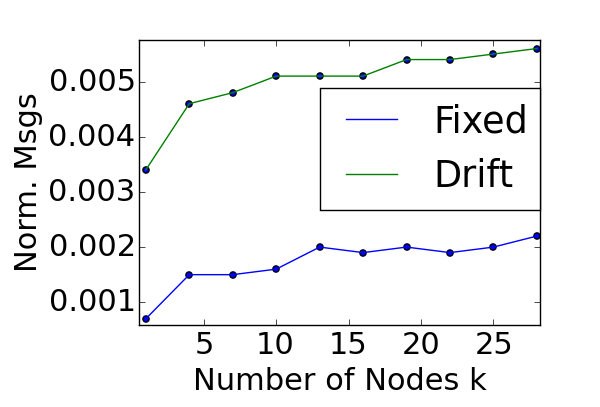
\includegraphics[width=\linewidth]{CommunicationOfFixedVsDrift/Nodes.png}
  \caption{Communication as a function of the number of nodes for fixed (blue) and concept drift including (green) datasets}\label{Nodes}
\endminipage\hfill
\minipage{0.4\textwidth}
    \centering
  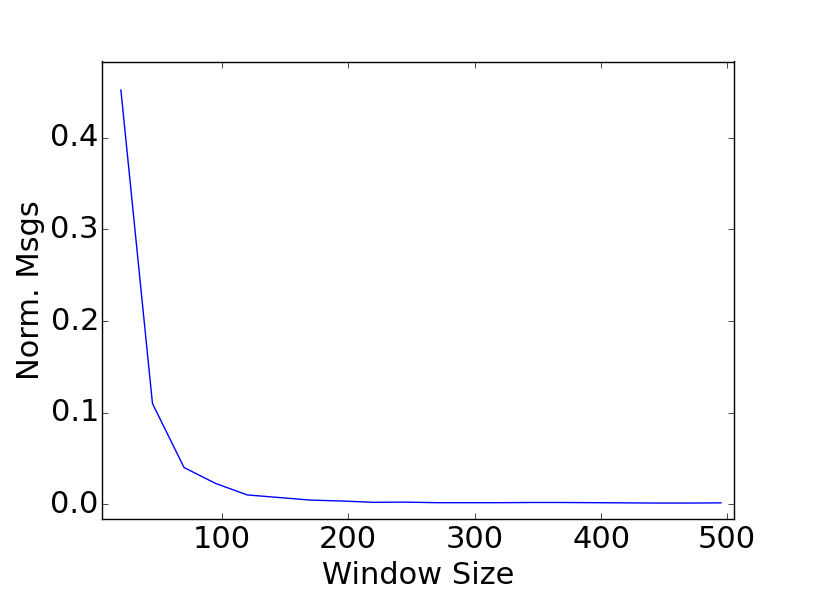
\includegraphics[width=\linewidth]{CommunicationOfFixedVsDrift/WindowSize.png}
  \caption{Communication as function of window size $W$ for fixed (blue) and concept drift including (green) datasets}\label{WindowSize}
\endminipage\hfill
\minipage{0.4\textwidth}
    \centering
  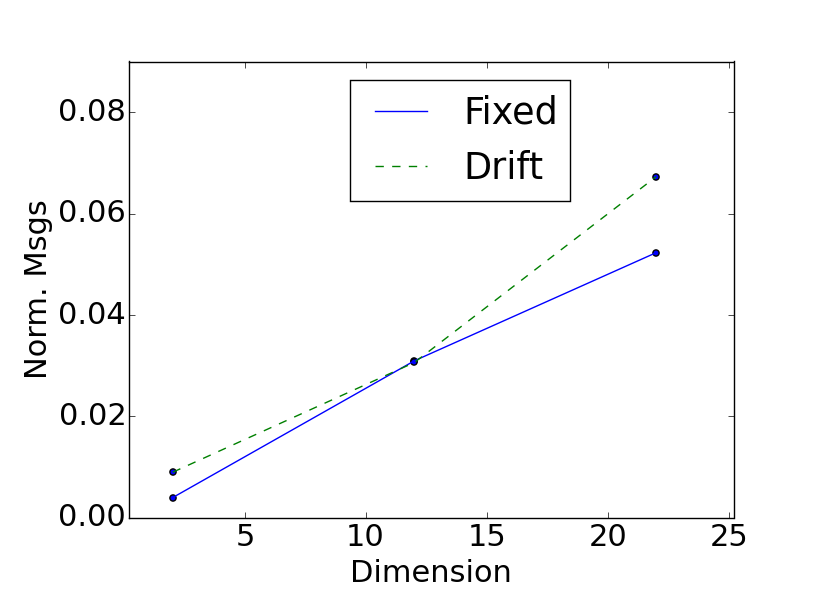
\includegraphics[width=\linewidth]{CommunicationOfFixedVsDrift/Dimension.png}
  \caption{Communication as a function of input dimension for fixed (blue) and concept drift including (green) datasets}\label{Dimension}
\endminipage
\end{figure}

\noindent\textbf{Window Size:}
Figure \ref{WindowSize} shows how communication decreases as a result
of enlarging the window size $W$.  One can increase the window size to compensate for other factors in the system that increase the communication. One of those is
noise (which is quantified in our context by the standard deviation of the
data generating distribution).

%\subsubsection{Noise}
%Figure \ref{Noise} shows normalized messages obtained for different
%noise magnitudes. The experiment shows that the drift grows with the noise, causing more %synchronizations (more communication). This result is not surprising, and the solution is to increase the window size.

Another parameter directly related to the window size is the dimension of the data. The number of samples required for accurate estimation of the covariance matrix grows with the dimension. In our settings, the number of training samples is linked to the window size. When window size is fixed, communication grows linearly with the dimension (see Figure \ref{Dimension}).



\begin{figure*}
	\centering
	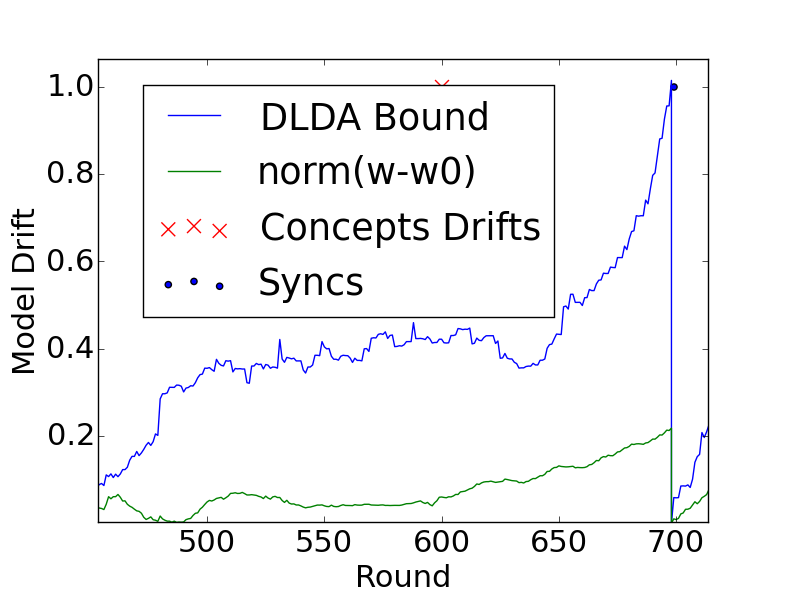
\includegraphics[width=\textwidth]{Usenet/DriftDetected.png}
	%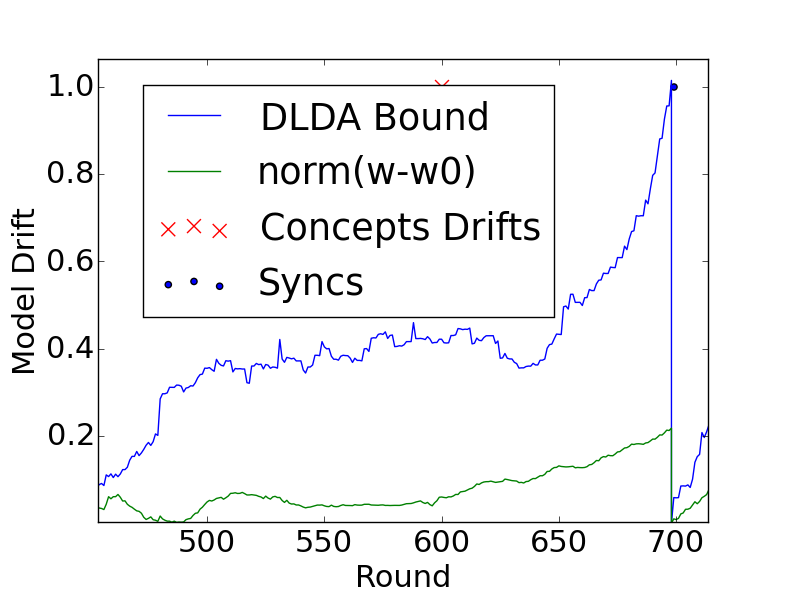
\includegraphics[width=\textwidth]{Usenet/DriftDetected.png}
	\caption{Comparison between maximal (over nodes) DLDA model drift (blue)
	and the true global model drift (green) for $k=2$, $W=450$.
	It can be seen that DLDA responds to the concept drift that occurs
	after 600 rounds (red dotted vertical line) and causes a synchronization in round 698 (blue dashed vertical line).}
	\label{usenet}
	\end{figure*}
\subsection{Real Data Experiments}
In this section we test the algorithm on three real data sets. The first
(USENET) is too small to test the probabilistic approach; thus we use this set only for the DLDA test.
The second (Power Consumption Monitoring) is a medium size dataset (it
is distributed over 36 nodes) and we test both DLDA and PDLDA on it.
The third (Gas Sensor Time Series Monitoring) is a big set(it is distributed over
100 nodes). The DLDA synchronization policy is too strict for a large number of nodes; hence we use this set only for the PDLDA test.

\subsubsection{Message Preference Monitoring --- Usenet}
The USENET dataset (~\citealt{usenet}) is a text dataset that simulates a stream of messages from three newsgroups (medicine, space, baseball); the messages are presented sequentially to a user, who then labels them as interesting or junk, according to personal interest. Attribute values are binary, indicating the presence or absence of the 128 informative words. The concept drift occurs from a change in the user's preference (from space to baseball). 
Figure \ref{usenet} shows the results of the DLDA algorithm with $W=450$ . The first 450 rounds over the data correspond to
the initialization phase and are omitted. During the next 50 rounds the DLDA model drift (the value is calculated using the left side of the inequality in Eq. \ref{eq:convexBound}) increases due to noise in the data; there is
no concept drift. From round 500 to 600 the DLDA model drift is stable,
and again is due only to the noise. In round 600 there is a concept
drift.
From this point both the DLDA model drift and the true model drift increase until the synchronization in round 698.
\subsubsection{Power Consumption Monitoring}
The Power Consumption dataset  (~\citealt{powerSupply}) contains the hourly power supply of an
Italian electric company as recorded from two sources: power supplied
by the main grid and power transformed from other grids.
This stream contains three-year power supply records
from 1995 to 1998, and our learning task is to predict which hour (1 out of 24 hours) the current power supply belongs to. The concept drift in this stream
is mainly caused by such factors as season, weather, time of day,
and the differences between working days and weekend.
We demonstrate the algorithms on the following binary classification problem:
given a power supply measurement, decide whether it corresponds to night or day.
This dataset is an example of gradual concept drift (seasons do not
change abruptly).
Figure \ref{PowerSupplyFigures} depicts the results of the DLDA
and PDLDA algorithms. For a small number of nodes, $k=4$, and for large
window size, $W=5000$, DLDA requires only 0.003 normalized messages.
For a more distributed system, $k=36$, and a smaller window
size, $W=600$, DLDA requires 0.09 normalized messages. For PDLDA with
$k=36$ and $W=600$ and a violation threshold (VT) of 50\%, PDLDA
requires 0.02 normalized messages, much better than DLDA in the same setting.

\begin{figure}[ht!]
    \centering
    \begin{subfigure}[b]{0.5\textwidth}
        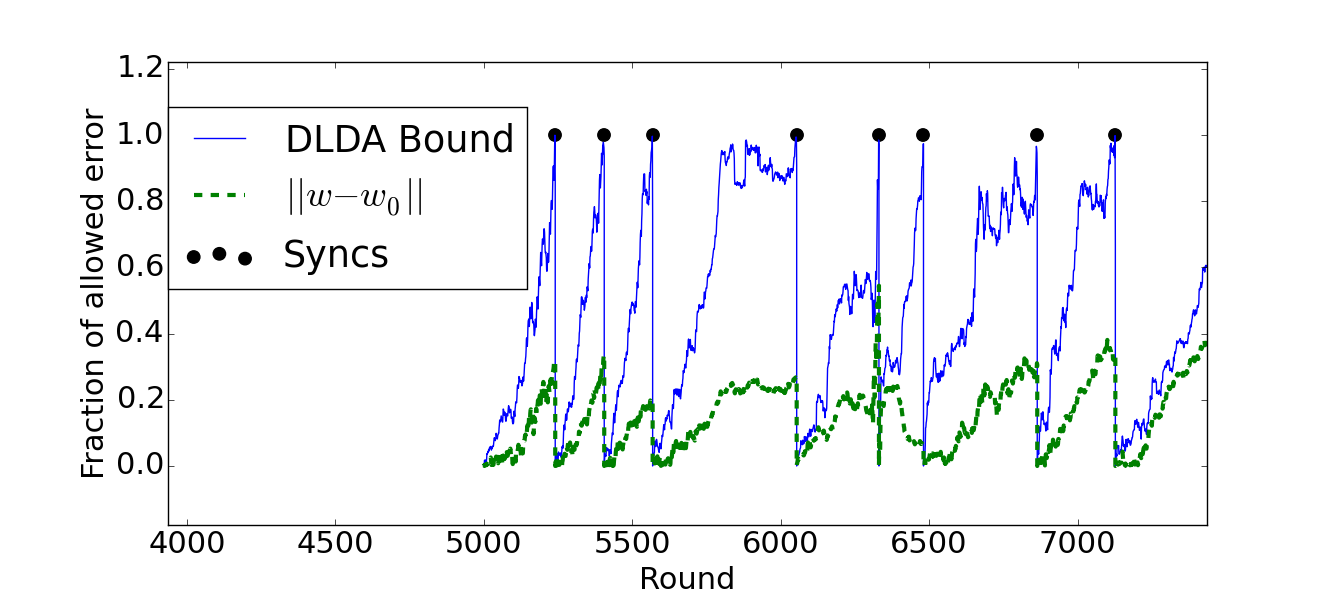
\includegraphics[width=\textwidth]{PowerSupply/4nodes.png}
        \caption{k=4, W=5000, VT=0}
    \end{subfigure}

    \begin{subfigure}[b]{0.5\textwidth}
        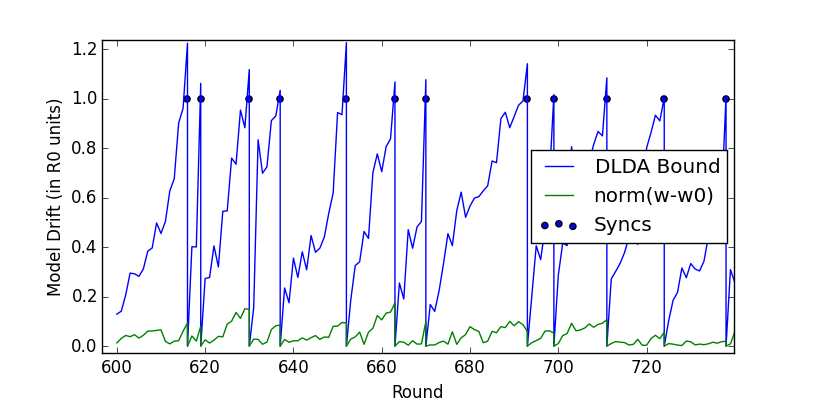
\includegraphics[width=\textwidth]{PowerSupply/36nodes.png}
        \caption{k=36 Nodes, W=600, VT=0}
    \end{subfigure}

    \begin{subfigure}[b]{0.5\textwidth}
        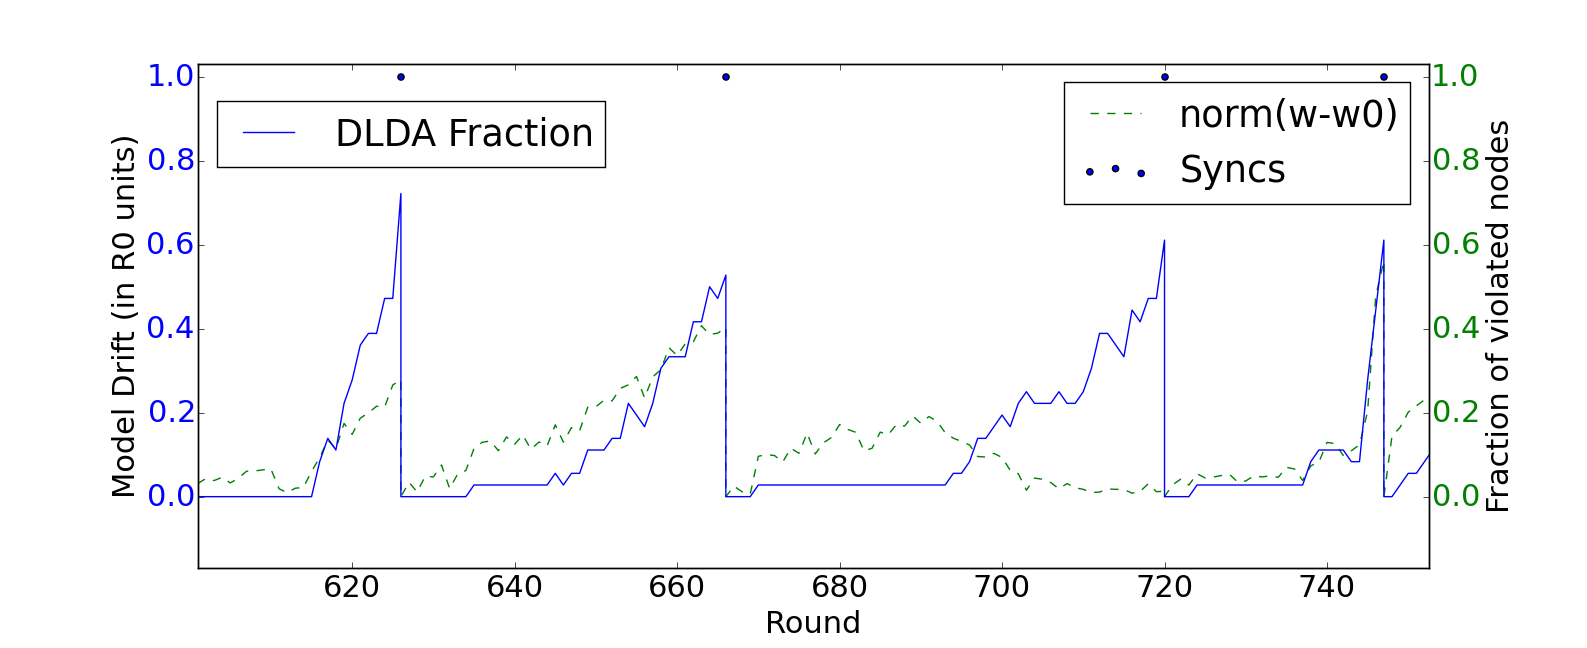
\includegraphics[width=\textwidth]{PowerSupply/36nodesProb.png}
        \caption{k=36 Nodes, W=600, VT=18}
    \end{subfigure}
    \caption{The top and the center figures show the DLDA algorithm on the Power Supply data set for a small (top) and large (center) number of nodes. The blue line represents the value of the local bound expression, corresponding to the node with the maximum value. The green line shows the model drift (normalized by the threshold); the model is computed after the data was aggregated from all nodes. The bottom plot shows the results of the PDLDA on the same dataset. The blue line in the bottom plot represents the fraction of violated nodes.}\label{PowerSupplyFigures}
\end{figure}

\subsubsection{Gas Sensor Time Series Monitoring}
\begin{figure*}[h]
\centering
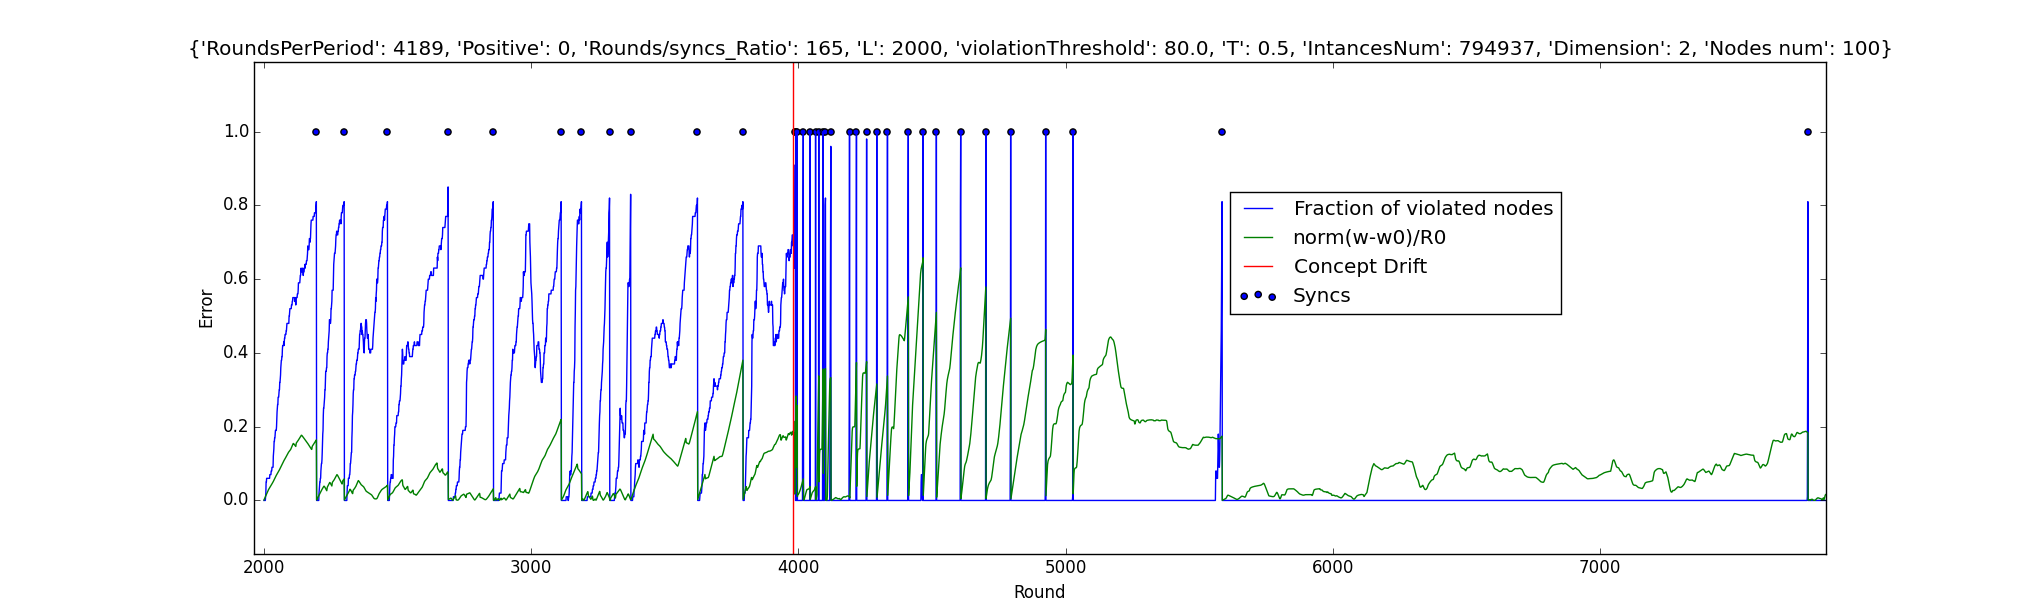
\includegraphics[width=\textwidth]{BigGas/overTime100k.png}
\caption{Demonstration of PDLDA on the Gas Sensor dataset.
A comparison between the true model drift (green) to the fraction of the nodes that
are violated in the current round (blue).
The experiment is configured for k=100 nodes, and the violation threshold is
VT=80.}
\label{BigGasOverTime}
\end{figure*}
Data in this experiment (~\citealt{bigGas}) consists of measurements collected
by an array of 16 chemical sensors in a lab, recording at a sampling
rate of 100Hz for 24 hours, resulting in 8378504 data points for each sensor.
During the first 12 hours the task is to detect the presence of carbon monoxide
(CO) in a mixture of chemicals, and from the 13th hour the task is to detect the presence of methane, which corresponds to an abrupt concept drift.
Figure \ref{BigGasOverTime} demonstrates the results of PDLDA algorithm.
First, we can observe that the fraction of violated nodes (shown in blue) correlates with the true model drift (shown in green). Second, we can see two patterns of behavior, which are separated by an abrupt switch in the data  (marked by the vertical red line). Before the switch,  the synchronization occurs every 150 rounds, and after the switch, it goes down to every 50 rounds. There is a transition period of about 1000 rounds that follows the point of the data switch. In this interval, the sliding window mixes the old (before switch) data and the new (after the switch) data, but once the window aggregates enough data, the algorithms stabilizes and reduces the communication requirements.   This experiment shows that the PDLDA algorithm detects the abrupt change in the data and adapts to the new conditions after a short period of time.
\section*{Conclusions}
We introduced the first communication-efficient monitoring algorithm for a linear classifier model that monitors the
models itself, but does not require knowledge of the global model at the local nodes.
As long as all nodes meet their local condition, the
global model is guaranteed to be valid. Our algorithm has important benefits:
\begin{itemize}
  \item Our method works with distributed data in a communication efficient way.
  \item Monitoring the model as opposed to monitoring the misclassifications allows for early detection of the concept drift misclassification occurs.
  \item Our algorithm is privacy aware in the sense that it preserves privacy of the data at each node from other nodes.
\end{itemize}

We evaluated the theoretical scheme -- DLDA,  and its probabilistic version -- PDLDA, on three real data sets.
For a small number of nodes we used DLDA with its theoretical guarantee, and for a greater number of nodes we used
PDLDA. We showed that the proposed scheme outperforms PER: it maintains a smaller Euclidean distance between
the last computed model and the current true model with a lower volume of communication.

This work is the first step in designing communication-efficient algorithms
with theoretical guarantees for monitoring classification models over dynamic distributed data
streams. 
Since we link the monitoring algorithm with the
hypothesis class and the learning algorithm, each classifier type should be
studied in depth.
Alternatively, a monitoring method could be developed for a given
hypothesis class, independent of the training algorithm.
One of the future directions is to extend the proposed framework to
ensembles of linear classifiers and neural networks, including deep learning networks.
An orthogonal, but important research direction is to analyze the
privacy aspect of the proposed algorithm and try to adjust the proposed
scheme in order to provide better privacy of the local data.

% BibTeX users please use one of
\bibliographystyle{abbrv}
\bibliography{bib}   % name your BibTeX data base
\nocite{*}

\begin{appendix}
To find a convex subset C satisfying the condition of Eq. \ref{convex},
we first define the operator norm:
\begin{definition}
Let $A$ be a matrix. Its operator norm, or
spectral norm, hereafter just norm, is defined as:
\begin{equation}
\Big \| A \Big \| = \sup_{x \neq 0}\frac{||Ax||}{||x||}.
\end{equation}
\end{definition}

\begin{lemma} \label{lemma:newman}
If A is square and $\Big \| A \Big \| < 1$, then
\begin{equation*}
\Big \| (I+A)^{-1} \Big \| < \frac{1}{1- \Big \|A \Big \|}.
\end{equation*}
\end{lemma}
The proof for this lemma can be found in \cite{gabel2015monitoring}.

\subsection{Convex Bound Proof}
We recall that $\mathcal{C}$ is the convex subset that satisfies
inequality \ref{convex} and $\mathcal{G}$ is the set of triplets
$(\Delta_s^i, \delta_p^i, \delta_q^i)$
 that satisfies the inequality \ref{eq:convexBound}.

\begin{lemma} \label{GinC}
%$\mathcal{G} \subseteq \mathcal{C}$:
\begin{equation}
\begin{split}
(||B_0^{-1}\delta|| + (||w_0||+R_0)(\Big \|B_0^{-1}L\Big \|+\Big \|B_0^{-1}M\Big \|) \\
 \leq R_0) \Rightarrow (||w-w_0|| \leq R_0).
\end{split}
\end{equation}
\end{lemma}

\begin{proof}
We can write the sphere condition in terms of $B_0, \Delta, u_0$ and $\delta$ using the triangle
inequality:
\begin{equation} \label{in}
\begin{split}
||w-w_0|| & = \ ||(B_0+\Delta)^{-1}(u_0+\delta) - B_0^{-1}u_0|| \\
& < ||(B_0+\Delta)^{-1}\delta|| \\
& \ \ + ||((B_0+\Delta)^{-1} - B_0^{-1})u_0||.
\end{split}
\end{equation}

We split the right side of the last inequality into two parts:
\begin{equation}  \label{e1e2}
\begin{split}
& E_1:= ||(B_0+\Delta)^{-1}\delta|| \\
& E_2:= ||((B_0+\Delta)^{-1} - B_0^{-1})u_0||.
\end{split}
\end{equation}
Under the assumption of $||B_0^{-1}\Delta||\ \leq \ 1$,
it follows from lemma \ref{lemma:newman}:
\begin{equation} \label{e1e2In}
\begin{split}
& E_1 \leq \frac{||B_0^{-1}\delta||}{1-\Big \|B_0^{-1}\Delta\Big \|} \\
& E_2 \leq  \frac{|| B_0^{-1}\Delta w_0||}{1-\Big \|B_0^{-1}\Delta\Big \|}.
\end{split}
\end{equation}
From norm properties we get:
\begin{equation} \label{CS}
||B_0^{-1}\Delta w_0||  \leq  \Big \|B_0^{-1}\Delta \Big \| ||w_0||.
\end{equation}
Substituting Eq. \ref{e1e2}, \ref{e1e2In} and \ref{CS} in Eq. \ref{in}, we
get:
\begin{equation}
\begin{split}
|| w-w_0 \parallel & \leq \ E_1+E_2 \\
& \leq \frac{||B_0^{-1}\delta|| + \Big \|B_0^{-1}\Delta\Big \|||w_0||}{1 -\Big \|B_0^{-1}\Delta \Big \|} \\
& \leq R_0.
\end{split}
\end{equation}
After rearranging the terms, we get
\begin{equation} \label{lostDenom}
||B_0^{-1}\delta|| + \Big \|B_0^{-1}\Delta \Big \| ||w_0||
\leq R_0(1 -\Big \|B_0^{-1}\Delta\Big \|).
\end{equation}
From the triangle inequality we can rewrite:
\begin{equation} \label{linQuad}
\Big \|B_0^{-1}\Delta\Big \| \leq \Big \|B_0^{-1}L\Big \|+\Big \|B_0^{-1}M\Big \|.
\end{equation}
And finally, combining inequalities \ref{lostDenom} and \ref{linQuad},
we get the following bound:
\begin{alignat*}{2} \label{convexBound}
&||B_0^{-1}\delta|| &+ (||w_0||+R_0)(\Big \|B_0^{-1}L\Big \|+\Big \|B_0^{-1}M\Big \|)  \leq R_0. \\
&
\end{alignat*}
\end{proof}

\begin{lemma} \label{GisConvex}
$||B_0^{-1}\delta|| + (||w_0||+R_0)(\Big \|B_0^{-1}L\Big \|+\Big \|B_0^{-1}M\Big \|$ is convex in $(\Delta_s,\delta_p, \delta_q).$
%$||B_0^{-1}\delta||$ is convex in $\delta$.
\end{lemma}
\begin{proof}
Multiplication by $B_0^{-1}$ is a linear operation and norm is a convex
operation. Therefore $||B_0^{-1}\delta||$ is convex in $\delta$.
%\end{proof}

We recall that:
\begin{equation*}
L:= \Delta_S - p_0\delta_p^T - \delta_pp_0^T - q_0\delta_q^T - \delta_qq_0^T.
\end{equation*}
%\begin{lemma} \label{L}
%$||B_0^{-1}L||$ is convex in $\Delta_s, \delta_p$
%and $\delta_q$.
%\end{lemma}
%\begin{proof}
$L$ is linear in $(\Delta_s, \delta_p)$ and therefore $\Big \|B_0^{-1}L\Big \|$ is convex in these variables.

%\end{proof}

We recall that:
\begin{equation*}
M:= - \delta_p\delta_p^T - \delta_q\delta_q^T.
\end{equation*}

%\begin{lemma} \label{M}
Whats is left to prove is that $\Big \|B_0^{-1}M\Big \|$ is convex in $(\delta_p, \delta_q)$.
%\end{lemma}
%\begin{proof}
\\From the definition of operator norm, we can rewrite the function as:
\begin{alignat*} {2}
\Big \|M \Big \| & = && ||B_0^{-1}(\max_{||u||=1}{\{u^T \delta_p\delta_p^T u\}} +
\max_{||u||=1}{\{u^T \delta_q\delta_q^T u\}})||\\
& = && ||B_0^{-1}(\max_{||u||=1}{\{||u^T \delta_p||^2\}} +
\max_{||u||=1}{\{||u^T \delta_q||^2\}})||.
\end{alignat*}
\\We observe that max over a finite number of convex functions is also a convex
function, and since multiplication by a matrix and the norm
operation preserve convexity, this concludes the proof.
\end{proof}

\begin{corollary}
From Lemmas \ref{GinC} and \ref{averages} we conclude that $\mathcal{G}\subseteq \mathcal{C}$. From Lemma \ref{GisConvex} we conclude that and $\mathcal{G}$ is convex, this completes the proof of Lemma \ref{convexBound}.
\end{corollary}
\end{appendix}
\end{document}
% end of file template.tex

